\chapter{Robot Navigation using ROS} \label{ch:BaseWork}


%%\section{Introduction}
When it comes to navigation we need a wide variety of modules that interconnected produce an intelligent system that makes the robot go from one point to another while avoiding obstacles and being well localized. 
The first problem that needs to be taken into account is where the robot is, for that we require map for a global reference. The second issue is finding the best route to a predefined goal. For that various algorithms and systems are already proposed and ready for use.
%For that we will try to define how we can produce a suitable navigation module for a given platform using state of the art algorithms and modules. First an overview of Robot Operating System (ROS) framework is presented. After that some navigation concepts are explained with further detail in path planning and motion control case. And finally how the \ac{ROS} navigation stack combats this problems.

\section {ROS}
Creating software for robotic applications is not an easy task to do from scratch. It usually involves very complex code to achieve even the simplest applications due to the wide variety of hardware and data that robots rely on. \ac{ROS} \cite{ros} fixes this issue by being a general purpose framework for robotics. Despite its name, it is not an operating system, being more a kind of middleware, since it  handles communication between programs in a distributed system. You can either construct one program that does all the computation needed in your application or you can have sub programs with each one having a specific functionality, the latter being often preferred.

\ac{ROS} provides hardware abstraction, tools for introspection, message-passing and more. Also it is open source which means we can use them for virtually any means which we deem necessary for the development of our application, for example adapting pre established code for a specific case. This greatly facilitates the entrance of new developers to learn and do research in the field of robotics.
\subsection{ROS architecture}
The \ac{ROS}  architecture is based on a peer to peer network between processes usually referred to as \textit{Computation Graph} \cite{packt}. This architecture is comprised by different concepts that we define bellow:
\begin{itemize}
\item \textbf{Nodes} - A node can be defined as a process or piece of software  that performs some type of computation. In \ac{ROS}, for a typical application there are various nodes running in parallel that pass information between each other. For example  controlling the robot movement given the input image of a camera,  requires a node to act as a driver between the camera firmware and the ROS environment. Then there could be a node that processes the image further using ROS pre established software and finally given the processed information a different node will calculate the velocity of the robot and transmit them to the wheels of the robot. 
\item \textbf{Messages} - \ac{ROS} uses defined data structures  called messages to represent information. This makes it so \ac{ROS} tools can generate the appropriate source code in the selected language (C++ or phyton in this case). Each message can be broke down into more messages and so one and so forth until we arrive at the primitive data types of the given programming language. 
\item \textbf{Topics} - 
%Nodes communicate by publishing or subscribing  to topics using the  messages and in the end we get a fully alive system that performs some type of application we want. 
Nodes can send messages by publishing to a topic or receive them by subscribing to a topic. For example a node can be subscribed a velocity message and then after some data processing publish a smoothed version of it into another topic.  
\item \textbf{Master} - Provides registration and naming for each node (helps nodes find each other). It is also responsible for organizing communication between nodes. Finnaly it also provides the \textbf{Parameter Server} (described bellow).
% V
\item \textbf{rosout} - This can be viewed as the ROS equivalent of stdout. This acts as a log reporting mechanism which is useful when debugging large amounts of code.
\item \textbf{Paramater Server} -In this server \ac{ROS} tracks different paramater values defined by the running application. It is useful for setting or getting different parameters dynamically without having to restart the application.

%X
\end{itemize}
Figure \ref{fig:rosgraph} gives a brief overview of how each of these concepts are put together and  generate the ROS  computation system.

\begin{figure}[ht!] 
\centerline{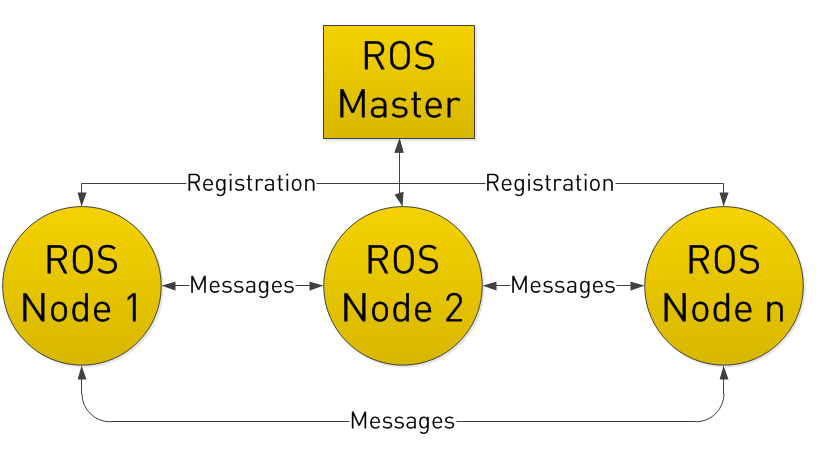
\includegraphics [width=0.6 \textwidth]{imgs/chapter3/rosgraph2.png}}
\caption[ROS communication architecture overview]{ROS communication architecture overview adapted from \cite{rosbasics}}
\label{fig:rosgraph}
\end{figure}


\subsection{ROS tools}
Now that we described the inner workings of \ac{ROS} we can use its tools to retrieve and analyze information regarding it. We will use the following \ac{ROS} tools:
\subsubsection{rviz}
\textbf{Rviz} is a graphical interface that allows 3D visualization environment that allows the view of the different components of \ac{ROS} like the robots frame transforms, the map, pointclouds, visualization markers etc...
\subsubsection{rosbag}
 Rosbag will subscribe to one or more topics and the serialized message data will be stored in a file as it is received. These files are called "bags" and contain information about all the \ac{ROS} topics chosen and can be played back at a predefined rate and can be started in any moment.
%\textbf{Rosbag} enables the recording of topics into a file that can be replayed in the future. By running this tool all the information regarding a the ROS structure is stored in a given time frame. This include the nodes, topics and messages that are passed along the way. 
%It is useful to store information and then running it again at the desired time and frequency rate we want.
\subsubsection{rqt_graph}
To understand how the various nodes and topics are interconnected the use of \textbf{rqt_graph} is the best for this case. It can be used to produce an image of all of them and how they communicate between each other
\subsubsection{Command Line tools}
In this section we will highlight some of the command line tools in \ac{ROS} that we used in this work.
\subsubsection*{Running ROS Systems}
\begin{itemize}
    \item \textbf{roscore} - this launches a process that the ROS System needs in order to properly setup communication between nodes. It starts the \ac{ROS} Master, Paramater Server and rosout. Using \textbf{roslaunch} will automatically run a roscore if it was not initiated before. 
    \item \textbf{roslaunch} - Used for running multiple ROS nodes as well as setting parameters in the server. This is done by launching ".launch" files that tell which nodes to load, which paramaters to set and what machines it will be used on.
    \item \textbf{rosrun} - Allows you to run a specific exacutable in a predetermined package.
\end{itemize}
\subsubsection*{Debugging and interacting with the \ac{ROS} system}
\begin{itemize}
    \item \textbf{rostopic} - is used for displaying debug information and interact with a given topic. This may be the messages published by a topic, finding a topic by its type, showing information about a topic, listing all the topics in the \ac{ROS} system. among other things.
   % \item \textbf{rossrv}
    \item \textbf{rosnode} - Can be used to display debug information about a node, regarding publications, subscriptions and connections.
    \item \textbf{rosparam} - Used for manage paramaters in the Paramater Server.
   % \item \textbf{rosmsg}

\end{itemize}

%%REVER ISTO




%\section{Architecture Overview}\label{ch:requirements}
\section {Navigation Concepts}
There are four main problems associated with robotic autonomous navigation. They are Mapping, Localization, Path Planning and Motion Control \cite{nav} as shown in Fig. \ref{fig:probNav} . 

\begin{figure}[ht!] 
\centerline{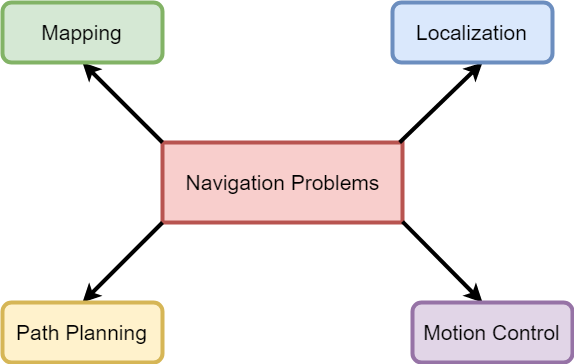
\includegraphics [width=0.6 \textwidth]{imgs/chapter3/navprobs.png}}
\caption{Problems regarding autonomous navigation}
\label{fig:probNav}
\end{figure}
Various algorithms have been developed over the years to combat these problems. 
%%Mapping

In regards to creating a suitable map,  \ac{ROS}  uses an improved version of  Rao-Blackwellized particle filters such as the ones described in \cite{grisetti2007improved}. This approach has proven to be an effective way to solve the \ac{SLAM} problem and will be used later on in this work to produce a valid map of our indoor environment.
%%Localization

With the grid map built we now need to estimate the robot's position in said map. 
An easy solution to this problem is relying on the robot's odometry information inferred by the robot's encoders and inertial sensors such as accelerometers and gyroscopes. This is called dead reckoning and is an easy and low cost solution for the localization problem. However since the sensor data is integrated over time, this leads to the accumulation of errors which make this approach not feasible for long navigation tasks. 
To fix this issue various algorithms were developed being the most popular ones based on particle filters. The \ac{AMCL} \cite{amclpaper} algorithm  is the standard choice in this case. It takes into account a group of particles, each one corresponding to a certain robot state (position and orientation in this case). As the robot moves the least probable states are filtered out and  the particles should over time converge on the actual position of the robot.  

Assuming the robot can localize itself on the map with a reasonable error we can start sending navigation goals to the robot. To reach the goal the robot must be able to find a path that optimizes the travel cost while avoiding obstacles. The outputted plan can vary depending on the algorithm used. This type of planning is often referred to as a global path planning that will be discussed further in a section \ref{ppmc} .

After an optimal plan is computed the final step is to determine the best velocity command that will be sent to the locomotion system.  The ROS navigation system follows a similar approach to the one used in \cite{gerkey2008planning}. A set of velocities are simulated during a given set of time and the corresponding predicted trajectories are  computed. This subject is often referred to as local path planner methods that will also be further detailed in the following section \ref{ppmc}.


\section{Path Planning and Motion Control}\label{ppmc}
 Obstacle avoidance is a major subject in robotics, as failure in this systems may result in crashes that have catastrophic consequences such as hardware being badly damaged or being completely nonfunctional. This subject is usually separated into two categories local path planning and global path planning \cite{foxdwa}.
 
 
 Global methods assume the environment is completely known a priori and can therefore compute an optimal safe path  around static obstacles using a variety of different strategies. These models prove to be very reliable for static environments. However these models are usually computational expensive which lead to very slow update times. For fast changing environments such as is in the case for highly populated indoor scenarios they prove to be insufficient. 
 To improve the quality of navigation capabilities, local path planning techniques are added to increase the responsiveness of the robot. These techniques have a much faster update time  since they use a smaller version of the world around them. However this type of approaches have trouble with local minimum cases where the robot can get stuck (for example the U-shape case).
\subsection{Global Methods for Path Planning}
Path planning is crucial for the robot to handle safe trajectory around obstacles. In this work the information regarding this obstacles is based on a grid map built by \ac{SLAM} and new observations retrieved by the robot's sensors.  Planning an optimal safe path can be done using a wide variety of methods like Visibility Graphs, Generalized Voronoi Diagram, and \ac{PRM} \cite{globalmethods}. However for in this work we will use the \ac{PRM} method. This method samples its environment and creates ano ccupancy graph. Then by inserting the initial position and the goal position the path can be computed using dijkstra, A* or Rapidly exploring Random Trees search algorithms . However, the \ac{ROS} navigation packages only use the first two so  we will only focus on these ones.


\subsubsection{Dijkstra algorithm}\label{djk}
Assuming we have an occupancy map we can now start to explain how does a robot compute the shortest path between the starting position and the end goal. Edsgar W. Dijkstra proposed an algorithm that solves this problem by computing the shortest cost path for a given occupancy graph. In our case we have cells on an occupancy grid map. The shortest path can be calculated doing the algorithm described in Figure \ref{fig:dalg}. 
\begin{figure}[ht!] 
\centerline{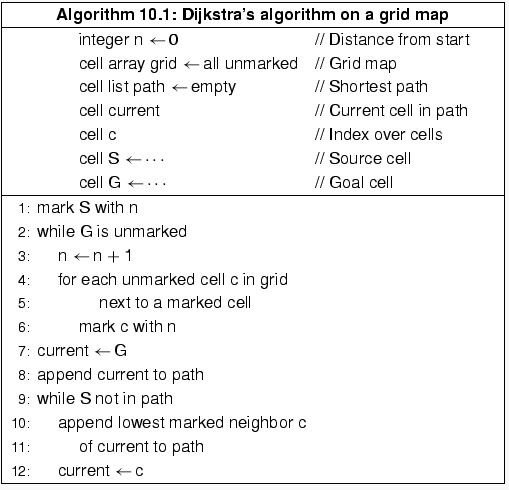
\includegraphics [width=0.7 \textwidth]{imgs/chapter5/Dalg.png}}
\caption[Dijkstra algorithm]{Dijkstra algorithm taken form \cite{Ben-Ari2018}}
\label{fig:dalg}
\end{figure}
Each cell is numbered with the number of steps it needs to get to the starting position. This continues until we reach the goal cell and we get the minimum path to reach it. However if we have a map with cells that have variable cost in the algorithm above we do not iterate $n$ with plus one, but with the cell cost. This makes it so for this case that  shortest path geometrically may not be the shortest path when the costs are taken into account.

\subsubsection{A* algorithm}\label{A*}
In the previous case we search for cells in all directions, however there is a more efficient way of doing it by adding more information. The A* algorithm besides the cost from the steps to the start position $g(x,y)$, it takes into account an extra \textit{heuristic function} $h(x, y)$ that gives a preferred direction for the search. 
%Not only does it take into account the cell cost but another value that corresponds to a given direction to be doing in  the search. 
The cost function in this case can be shown as:
\begin{equation}
    f(x,y)=g(x,y) + h(x,y)
\end{equation}
\subsection{Local Methods for Motion Control }
In contrast to global path planning where a large portion of the environment is generally assumed to be known local methods take into account a partial world view for motion planning capabilities. The most popular of this type of methods are \cite{inbookdwa}:
%cite this
\begin{description}
    \item [\ac{DWA}] -  \cite{foxdwa} Takes into account a substet of admissible velocities and the robot's dynamic constraints and simulates them for a given time frame outputting various trajectories. Then using these trajectories derives the best trajectory given a certain cost function.  
    \item [Trajectory Rollout]  \cite{gerkey2008planning} - Similar to the \ac{DWA} planner except the sampling method for the control space is different.
    \item [Elastic Band] - \cite{siegwart2011introduction} In this case bubbles are formed that are defined as the maximum local subset of free space around a given robot configuration that can be travelled without collision.
    Given these bubbles a set of "elastic bands" are connected to form a collision free trajectory from the initial position to the goal without collision. When it comes to avoid an obstacle that obstructs the global plan, this technique tends to deviate from it  minimizing the bubble band tension.
    \item [Timed elastic band] - \cite{rosmann2013efficient} This planner is an extension of the 'elastic band' that takes into account time intervals in between the robot's position and orientation. By doing this, and utilizing a  multiple objective optimization function, that takes into account the robot's acceleration and velocity limits with penalties and computes the best trajectory taking into account execution time, shortest path and clearance of obstacles it creates a suitable local planner that is suitable for avoiding dynamic obstacles.
    
    \item [Clothoid Tentacles] -  \cite{ffalia2015local} This is an empirical approach to the local path planning problem. It generates various "tentacles" and take the form of clothoids. It then chooses the best one taking into account the best obstacle clearance, curvature and distance to the global path planner. 
    
    \item [\ac{VFH}+] \cite{siegwart2011introduction} - For this approach a histogram of the ammount of obstacles in a certain direction is first created.Then using a cost function that takes into account the alignment of the robot towards the goal, the difference between the new direction and the current wheel orientation and the difference between the previously selected direction and the new direction is computed. The best trajectory is then chosen taking into account this information.
    
\end{description}
For our case study we will only study in detail the first two in detail since they are already implemented in ROS.
\subsubsection{DWA planner}\label{dwa}
The \ac{DWA} planner is the most standard approach when it comes to local path planning in \ac{ROS}. It outputs  rotational and translational velocities by generating multiple trajectories for different types of velocity sample search space and choosing the best one. The algorithm goes as follows \cite{inbookdwa}:
\begin{itemize}
    \item Start with a set of velocities pairs (translational and rotational) $\{(R_{vR_x},R_{ \omega_z}  )\}$ that are obtainable by the robot.
    \item Genarate in the form of arcs the projected trajectories obtained using the previous velocity sample space.
    \item Dismiss velocities that result in the robot colliding with an object in a given time frame. With this we are left of a subset of admissible velocities $V_a=(R_{vR_a},R_{ \omega_a})$ in which:
    \begin{equation}
         V_a=(R_{vR_a},R_{ \omega_a}) \Rightarrow \begin{cases}
    R_{vR_x} & 	\leq \sqrt{2*dist(R_{vR_x},R_{ \omega_z})*R_{\dot{v}_{xb}}}.\\
    R_{ \omega_z}  &  	\leq \sqrt{2*dist(R_{vR_x},R_{ \omega_z})*R_{\dot{\omega}_{zb}}}.
  \end{cases}
    \end{equation}
    Where $R_{\dot{v}_{xb}}$ and $R_{\dot{\omega}_{zb}}$ are the braking accelerations of the robot and $dist$ the distance to the closest obstacle found n the trajectory.
    
    
    \item Dismiss velocities that don't respect the robot's acceleration limits in a given simulated time frame. With this we are left with a subset of velocities called dynamic window $V_d=(R_{vR_d},R_{ \omega_d})$  in which:
    \begin{equation}
         V_d=(R_{vR_d},R_{ \omega_d}) \Rightarrow \begin{cases}
    R_{vR_x} & 	\in [R_{v_a}-R_{\dot{vR}_{x}}*t,R_{v_a} + R_{\dot{vR}_{x}}*t].\\
    R_{\omega_z} & 	\in [R_{ \omega_a}-R_{\dot{\omega}_{z}}*t,R_{\omega_a}+R_{\dot{\omega}_{z}}*t].\\
  \end{cases}
    \end{equation}
    \item Finally we choose  the most optimal trajectory and in consequence velocity pair taking into account a given objective cost function.
    \end{itemize}
\subsubsection{Trajectory Rollout} \label{tr}
The Trajectory Rollout planner follows the same logic as above but in this case the sampling method for the control space is different. In this a set permissible velocities
in each simulation is calculated including acceleration limits for the entire simulation time\cite{inbookdwa}.Instead of searching the space of feasible trajectories, we search the space of feasible controls. In Trajectory Rollout set of permissible velocities in each simulation is calculated including acceleration limits for the entire simulation
time, while in Dynamic Window Approach it is limited to one simulation step.
\section {ROS Navigation stack}
The ROS navigation stack is a set of software packages that properly combined can get a robot to navigate autonomously.
Figure \ref{fig:plans} shows an example of \textbf{turtlebot2} using the navigation stack to drive autonomously.
\begin{figure}[!htb]
    \centering
    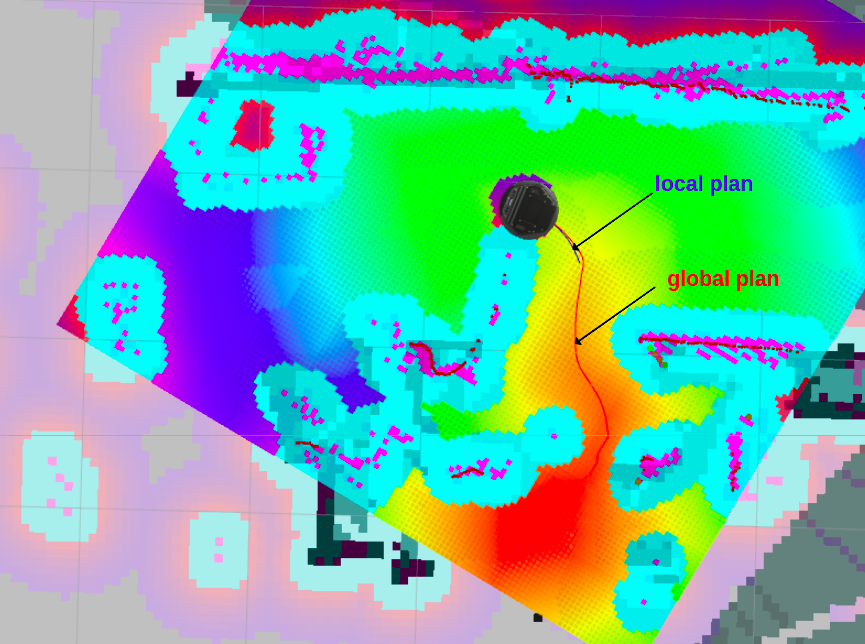
\includegraphics[width=\linewidth]{imgs/chapter3/nav.png}
    \caption[Rviz view of the ROS Navigation Stack]{Rviz displaying the ros navigation stack components while \textbf{turtlebot2} is navigating.}
    \label{fig:plans}
\end{figure}

\subsection{Requirements}
 Before running the \ac{ROS} navigation stack we first need to properly setup the robot to meet its requirements.
\subsubsection{Transform Configuration}
The Navigation stack requires that the relationships between the different frames must be published in \textbf{tf} or \textbf{tf\_static} topic. This makes it so the robot perceives what is around it correctly.
Figure \ref{fig:tf} shows all the frames and their transforms with each other for \textbf{turtlebot2}. However the main transforms that we need to worry about are between the sensors and the base link frame.
\begin{figure}[!htb]
    \centering
    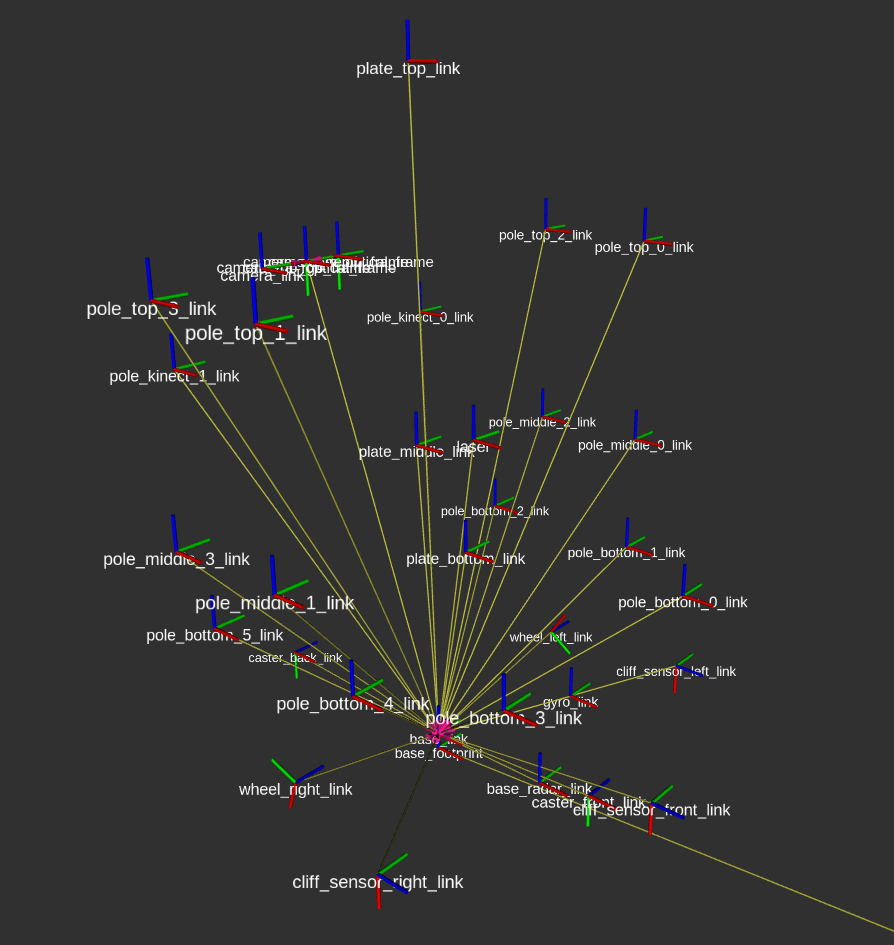
\includegraphics[scale=0.4]{imgs/chapter3/tf.png}
    \caption{Example of the transform relationships}
    \label{fig:tf}
\end{figure}

\subsubsection{Sensor sources}
To avoid obstacles we need some type of sensors that can detect them. Before running the stack we need to make sure they are publishing information.
This information needs to be in either a  \texttt{PointCloud2} or \texttt(LaserScan) message format.
Figure \ref{fig:sensors} shows an example of the published data from both in rviz.
\begin{figure}[!htb]
    \centering
    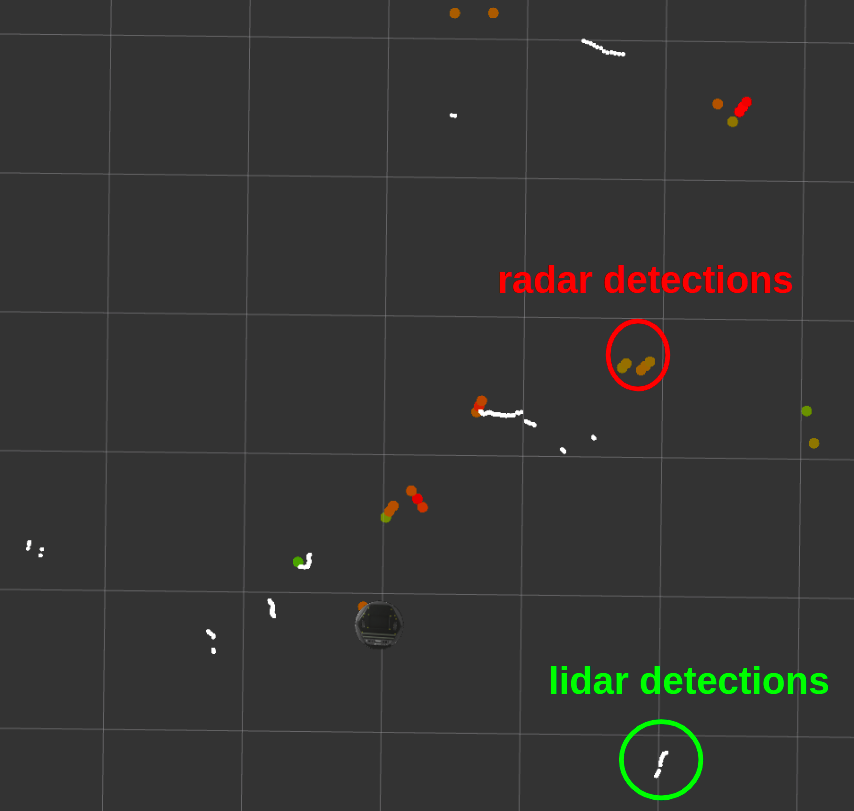
\includegraphics[scale=0.5]{imgs/chapter3/sensors2.png}
    \caption{Obstacle detections by both radar and lidar}
    \label{fig:sensors}
\end{figure}
\subsubsection{Odometry}
We need to have a rough estimation of the robot localization. Therefore we require a topic that publishes odometry information.
\subsubsection{Base Controller}
This module will subscribe to the velocity message outputted by the navigation stack and convert them into the appropriate motor commands to send to the mobile base that will actually make the robot move.
%%GARBAGE
\subsubsection{Mapping}
This part is not mandatory but it helps to have some sort of map being published to use as a global reference for the robot. It is used by \texttt{amcl} node to correctly localize the robot and to mark previously detected static obstacles when the map was built. Fig. \ref{fig:map} shows an example of a map that might be used by the ROS navigation stack.
\begin{figure}[!htb]
    \centering
    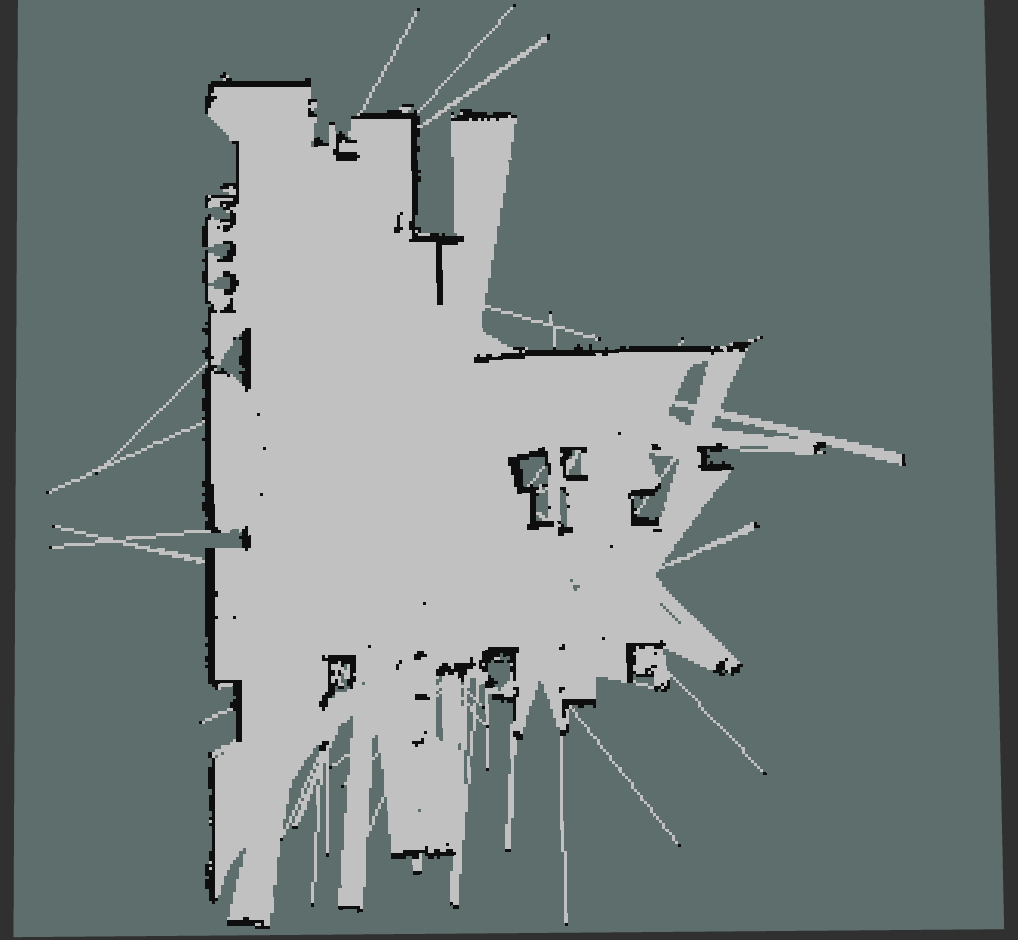
\includegraphics[scale=0.4]{imgs/chapter3/map2.png}
    \caption{Example of a map created in the IRIS laboratory}
    \label{fig:map}
\end{figure}
If the setup is done correctly we can now run the navigation stack.
\subsection{Navigation Node}
%%STUFF
Now that we have all the things we need for navigation we need an entity that actually processes all this information in an intelligent way to determine the best velocity command for the robot. This is done by the \texttt{move\_base } node and its peripherals.
Figure \ref{fig:navstack} shows an overview of the different components of the navigation stack \cite{movebase}.
\begin{figure}[!htb]
    \centering
    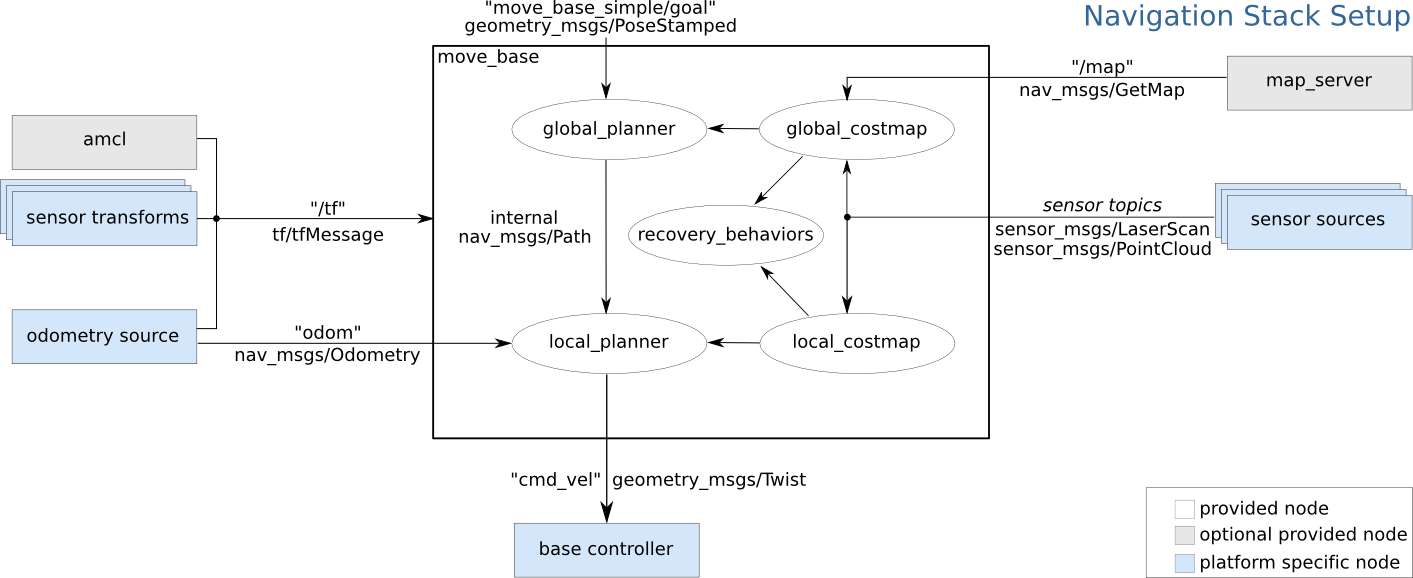
\includegraphics[width=\linewidth]{imgs/chapter3/navstack.png}
    \caption[Navigation stack block diagram]{Navigation stack block diagram taken from \cite{movebase}}
    \label{fig:navstack}
\end{figure}

The move base node links together the global and local planner as well as a local and global costmap to achieve the end goal provided by an action server. It also loads a set of determined recovery behaviors if the planners fail to produce a valid path. 

The global and local planners are plugins specified by the user. This choice will affect the behavior of the robot depending on the planners architecture and parameters. As of right now, it is integrated in \ac{ROS}  two global planners, the \textbf{navfn} and \textbf{global_planner}, and three local planners the \textbf{TrajectoryPlannerROS}, \textbf{DWAPlanner} and \textbf{carrot_planner}.

In this work it will be used \textbf{navfn} as our global planner and \textbf{TrajectoryPlannerROS} as our local planner.

\subsubsection{Global Planner}
 
The job of this component is to produce the best trajectory for a robot to take with limited amount of information given by the global costmap.
This plan can be updated when the robot gets stuck or by using a user specific frequency, the latter is usually preferred. The algorithms used to get this path are usually \textbf{dijkstra} or \textbf{A*} that are described in the previous sections \ref{djk} and \ref{A*}.

\subsubsection{Local Planner}
The local planner takes into account the trajectory given by the global planner and tries to compute velocity commands that follow it. However the path given may be to close to an obstacle detected and in order to avoid it the robot must deviate from the plan given to avoid collision. The function of the local planner is to avoid dynamic obstacles that appear while still trying to follow the global plan and goal. This type of local planner is usually \textbf{TrajectoryPlannerROS} or \textbf{DWAPlanner} that follow the explanation in the previous sections \ref{dwa} and \ref{tr} and uses the local costmap to do so. Bellow, we explain how \textbf{TrajectoryPlannerROS} generates the best trajectory using a determined cost function.

\subsubsection*{Getting the Best Trajectory}
The algorithm to get the best trajectory goes as follows:
\begin{enumerate}
    \item Discreetly sample the velocity space ($d_{vx}$ and $d_{vtheta}$)
    \begin{align*}
        & d_{vx}=(\texttt{max\_vel\_x}-\texttt{min\_vel\_x})/\texttt{vx\_samples}\\
         & d_{vtheta}=(\texttt{max\_vel\_theta}-\texttt{min\_vel\_theta})/\texttt{vtheta\_samples}
    \end{align*}
    \item For each sampled velocity predict its trajectory in a given time frame (\texttt{sim\_time}).
    \item Evaluate the cost of each trajectory  by using the value cost function
    \item Pick the one with lowest cost and publish the associated velocity.
    \item Repeat for a given rate (\texttt{controller\_frequency})
\end{enumerate}
\subsubsection*{Cost Function}
The cost function used to evaluate a trajectory is given by:
\begin{align*}
        \textbf{cost} = &
   \texttt{pdist\_scale} * \textbf{path\_dist}
   + \texttt{gdist\_scale} * \textbf{goal\_dist}\\
   &+\texttt{occdist\_scale} * \textbf{max\_obs\_cost} 
\end{align*}
where \textbf{path\_dist} is the distance from the endpoint of the trajectory to the global path in map cells, \textbf{goal\_dist} is the distance from the endpoint of the trajectory to the local goal (goal that is withing the local costmap taking into account the global plan)  in map cells, and \textbf{max\_obs\_cost} is equal to the \textbf{maximum obstacle cost} (given by the local costmap) of all the points along the trajectory.
Fig. \ref{fig:costcloud} displays an example of this values when the robot is navigating.
\begin{figure}[!htb]
    \centering
    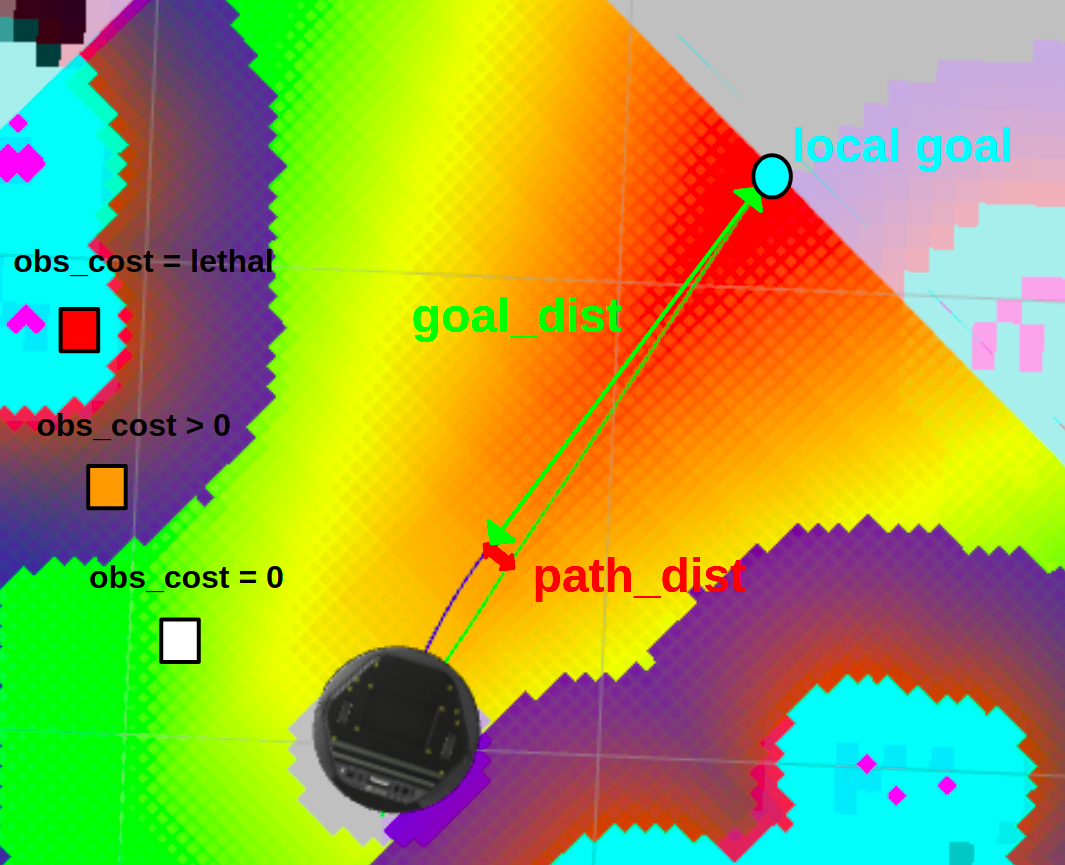
\includegraphics[width=0.8\linewidth]{imgs/chapter3/costcloud.png}
    \caption[Cost cloud published in rviz]{Cost cloud published in rviz. Red cells correspond to low cost and green cells correspond to a high cost}
    \label{fig:costcloud}
\end{figure}
\subsubsection{Local and Global Costmaps}
The global and local costmaps share the same class, the  \texttt{Costmap2DROS}. This class consists of a layered costmap that takes into account various layers defined by the user.

\subsubsection*{Available Layers}
\begin{itemize}
    \item \textbf{Obstacle Layer} - Marks objects retrieved from our sensor sources with lethal value. It also raytraces observations to clear out space.
    %Does more stuff
    \item \textbf{Inflation Layer} - Inflates the detected obstacles taking into account the robot radius and inflation radius. The closer the cells are from a lethal obstacle the more value they will have.
    %%....(needs explanation)
    \item \textbf{Static Layer} - Retrieves static information from the \textbf{/map} topic and marks them has lethal objects (Typically only used in global costmap).
\end{itemize}

Figure \ref{fig:layers1} shows how the combined layers produce the master costmap that will be used by the planners \cite{lu2014layered}.

\begin{figure}[!htb]
    \centering
    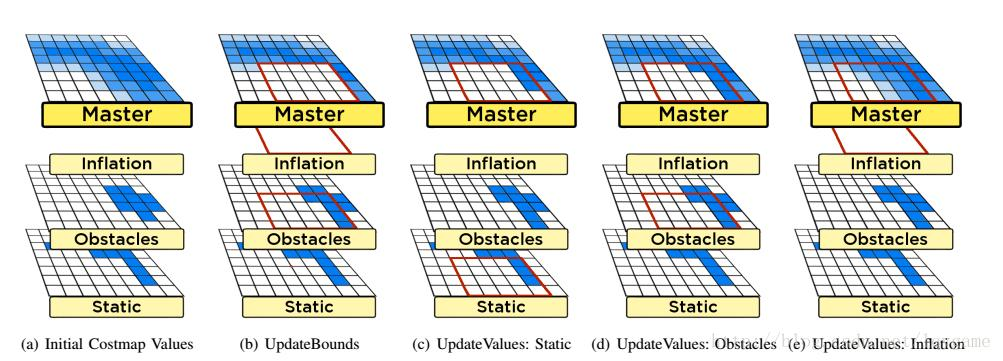
\includegraphics[width=\linewidth]{imgs/chapter3/layers1.png}
    \caption[Determination of the master costmap taking into account different costmap layers]{Determination of the master costmap taking into account different costmap layers from \cite{lu2014layered}}
    \label{fig:layers1}
\end{figure}
\section{Summary}
In this chapter we described the inner workings of the ROS framework and what tools can be used in order to develop a certain application. We also discussed what types of problems exist in regards to autonomous navigation. Finally we showed how the ROS navigation stack tackles these issues in order to construct a safe navigation module for a robot.


